% !TeX root = ../../progress-sem1.tex
% 3.x การออกแบบระบบ (System Design)
\section{การออกแบบระบบ (System Design)}
\begin{samepage}
  \subsection{Use Case Diagram}
  \thaijustify{
    แผนภาพกรณีการใช้งาน (Use case diagram) แสดงความสัมพันธ์ระหว่างผู้ใช้งานแต่ละบทบาทกับฟังก์ชันของแพลตฟอร์ม โดยแบ่งออกเป็น 4 ส่วน ได้แก่ ส่วน Authentication, ส่วนสร้าง two-alternative UI, ส่วนทดสอบการใช้งานและรับความเห็น, และส่วนสร้างรายงาน
  }
  \subsubsection{Authentication}
  \begin{figure}[H]
    \centering
    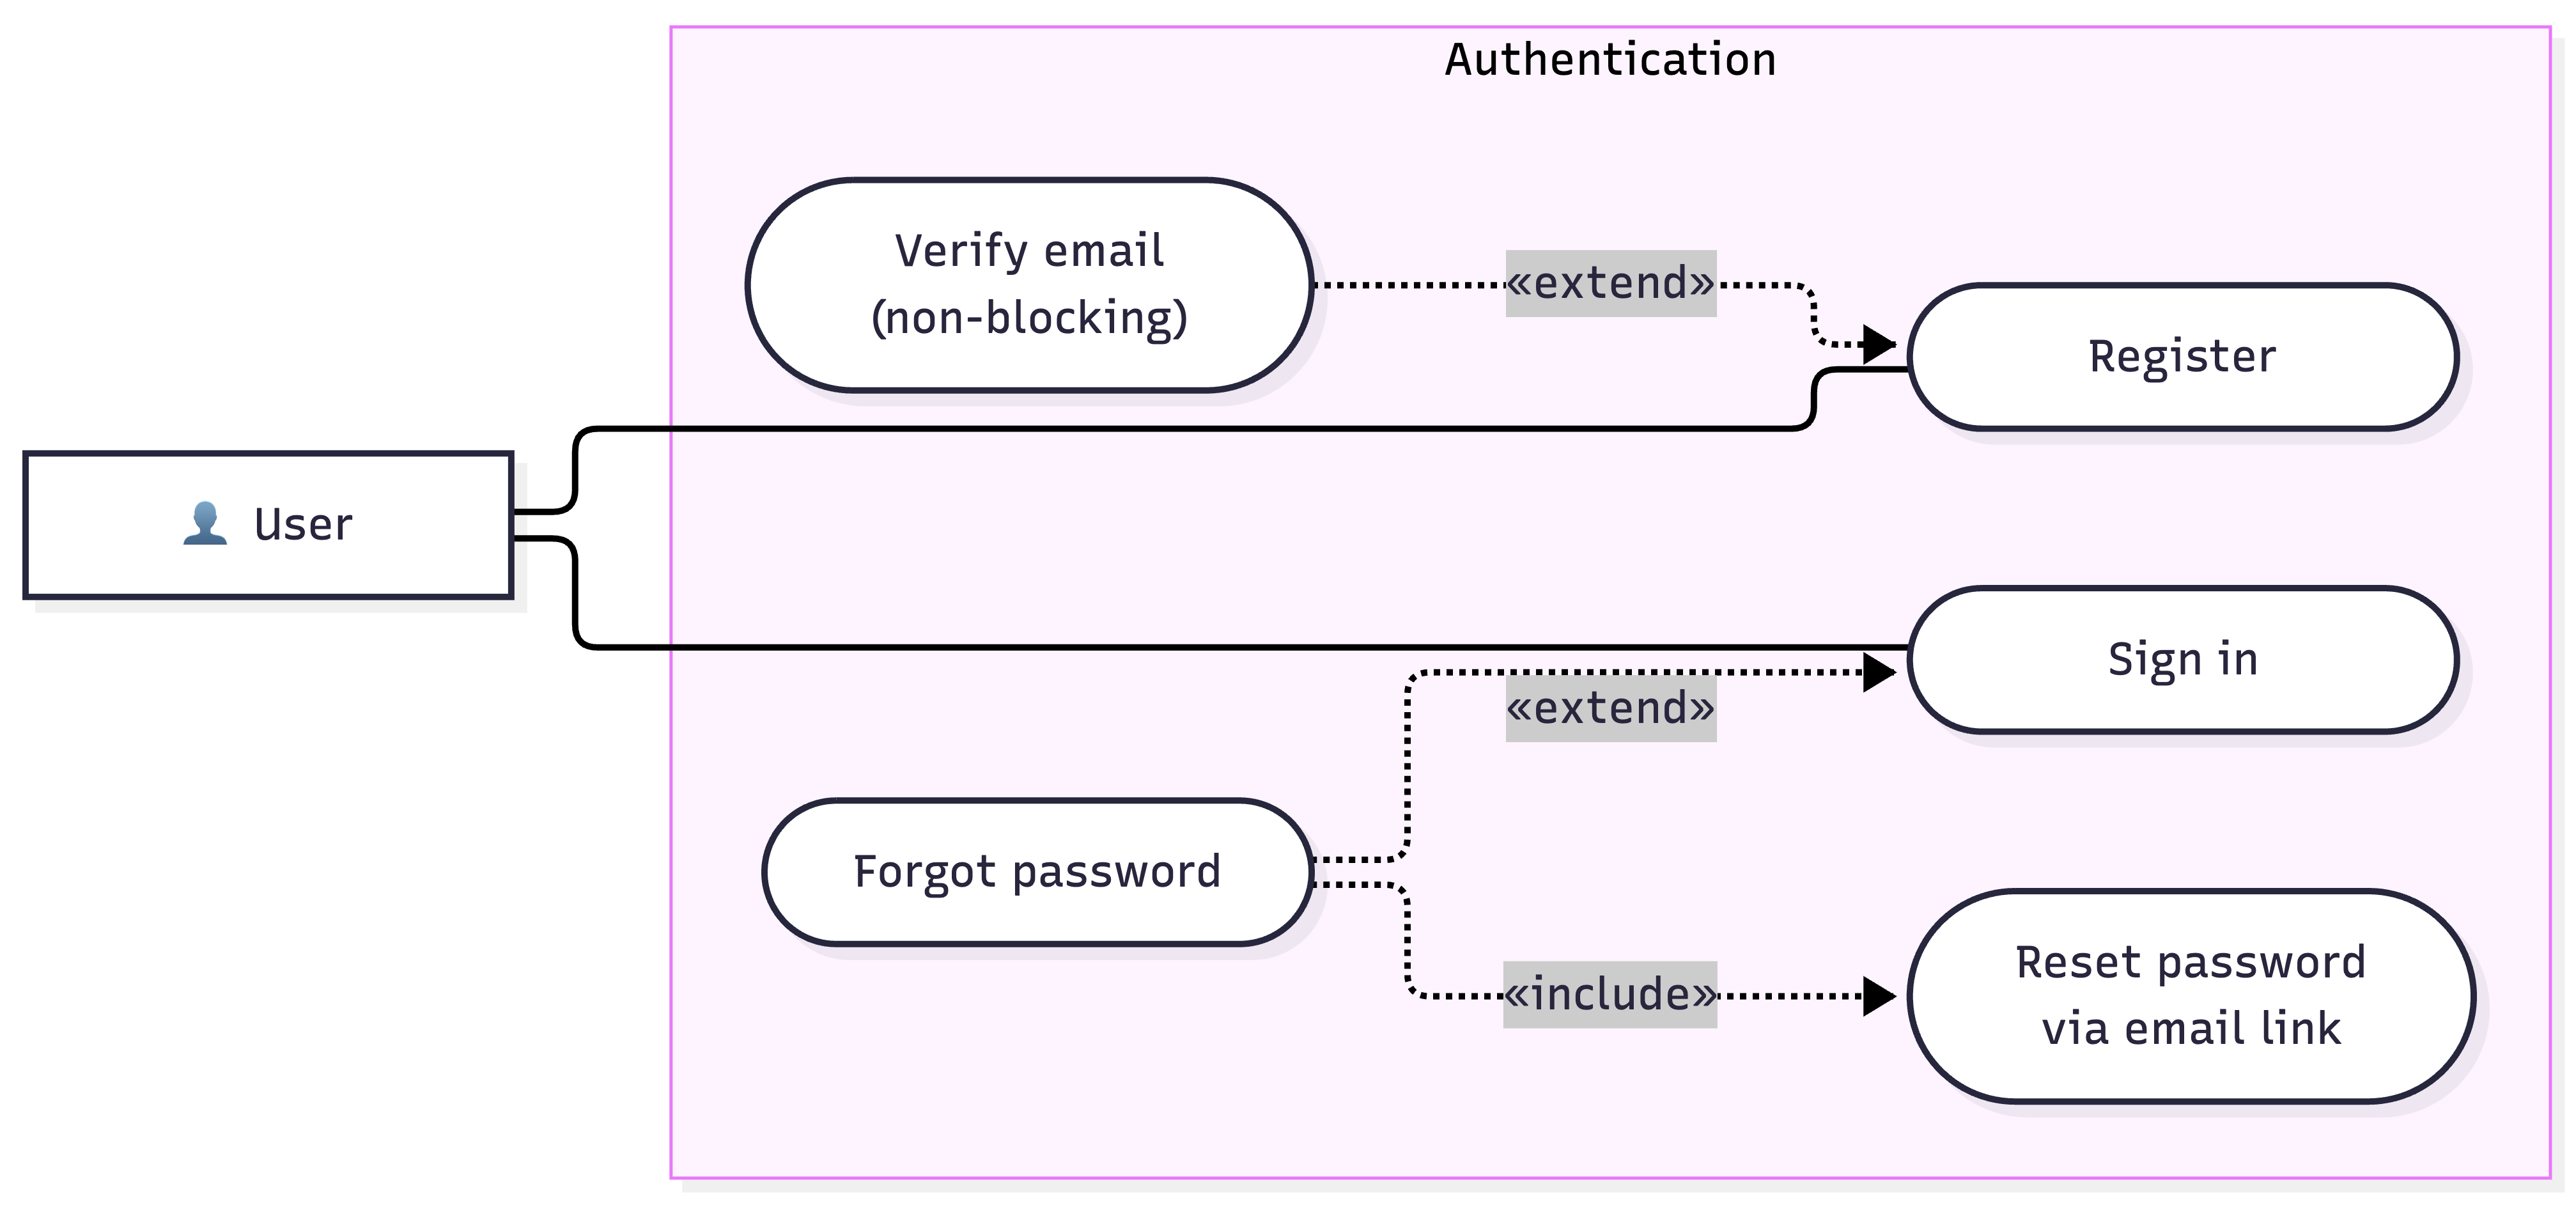
\includegraphics[
      width=0.6\textheight,
      height=\linewidth,
      keepaspectratio,
      origin=c
    ]{figures/ch3-methodology/UC-1.png}
    \caption{Use case diagram for authentication}
    \label{fig:UC-1}
    \thaijustify{ภาพแสดง Use Case ของระบบ Authentication โดยผู้ใช้สามารถสมัครสมาชิก เข้าสู่ระบบ และกู้คืนรหัสผ่านได้ โดยการยืนยันอีเมลเป็นขั้นตอนเสริมหลังการสมัคร และการรีเซ็ตรหัสผ่านดำเนินการผ่านลิงก์ที่ส่งทางอีเมล}
  \end{figure}
  \subsubsection{Designer: Project setup \& UI Generation}
  \begin{figure}[H]
    \centering
    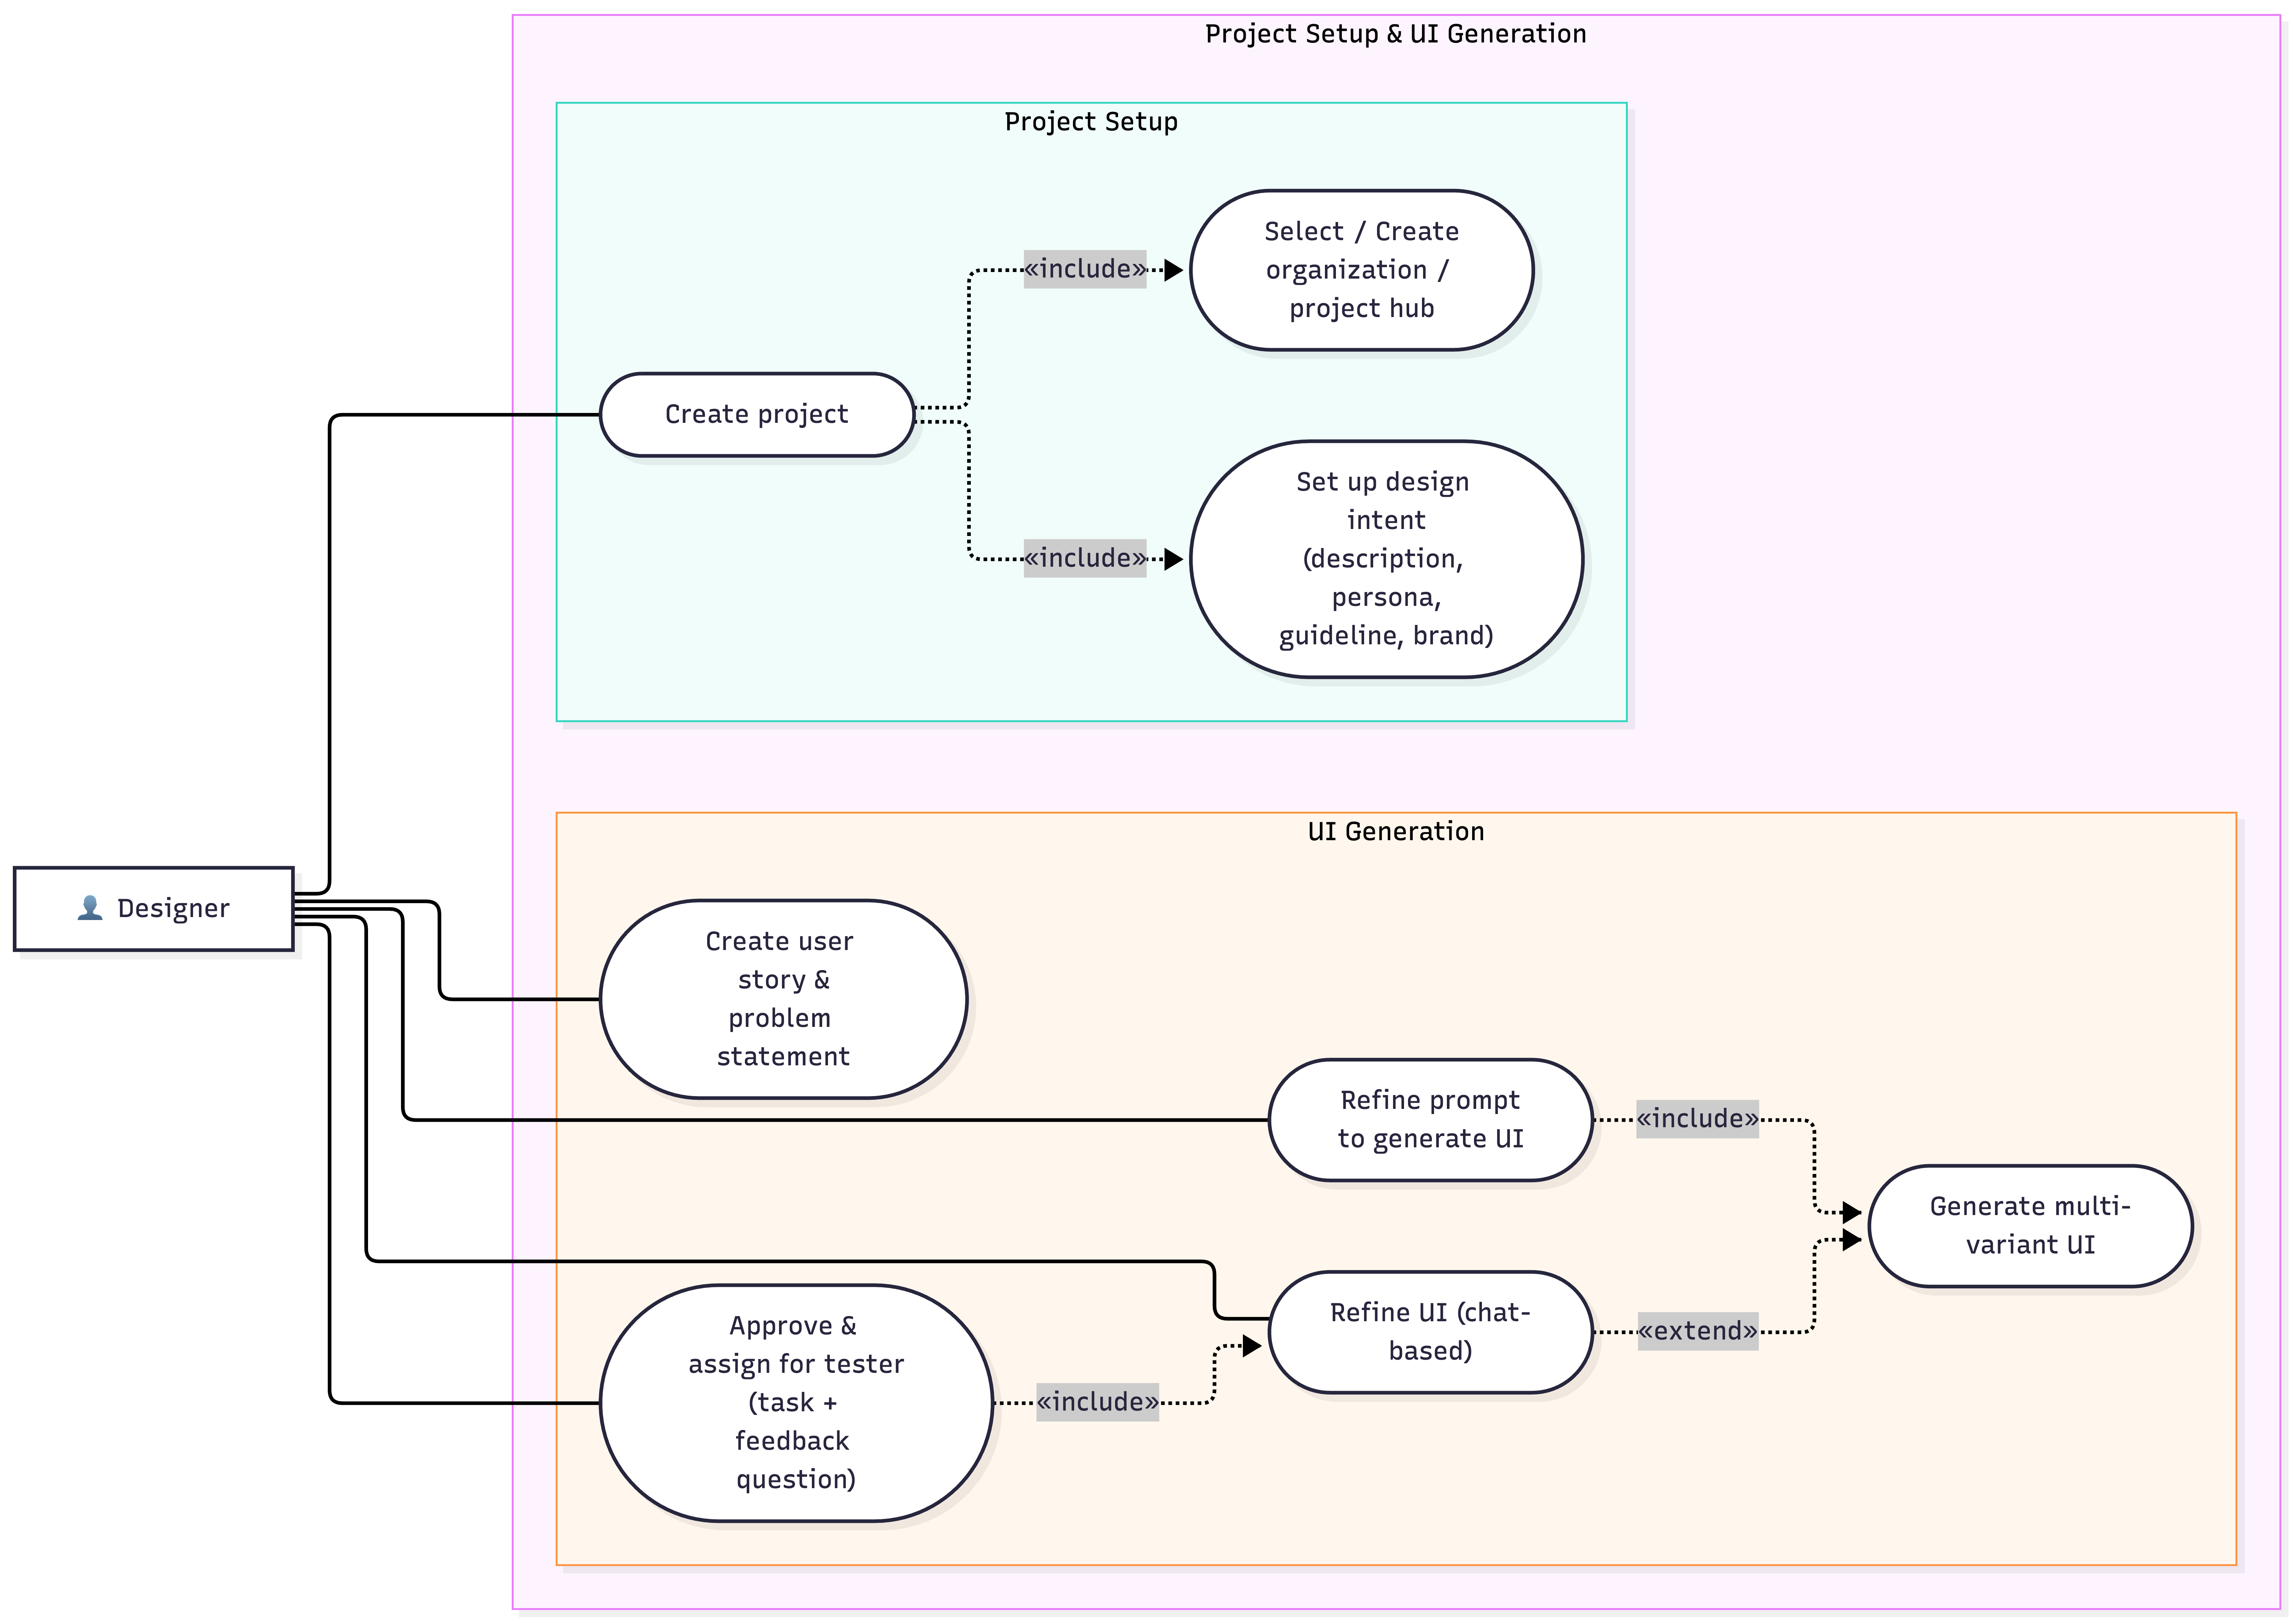
\includegraphics[
      width=0.6\textheight,
      height=\linewidth,
      keepaspectratio,
      origin=c
    ]{figures/ch3-methodology/UC-2.png}
    \caption{Use case diagram for Project setup and UI Generation}
    \label{fig:UC-2}
    \thaijustify{ภาพแสดง Use Case ของกระบวนการจัดเตรียมโครงการและสร้าง UI โดย Designer สามารถสร้างโครงการ กำหนด Design Intent สร้างและปรับแต่ง Prompt เพื่อสร้าง UI หลายรูปแบบ รวมถึงปรับแก้ UI และอนุมัติเพื่อส่งให้ผู้ทดสอบประเมิน}
  \end{figure}
  \subsubsection{Designer and Tester: Testing session and Feedback analysis}
  \begin{figure}[H]
    \centering
    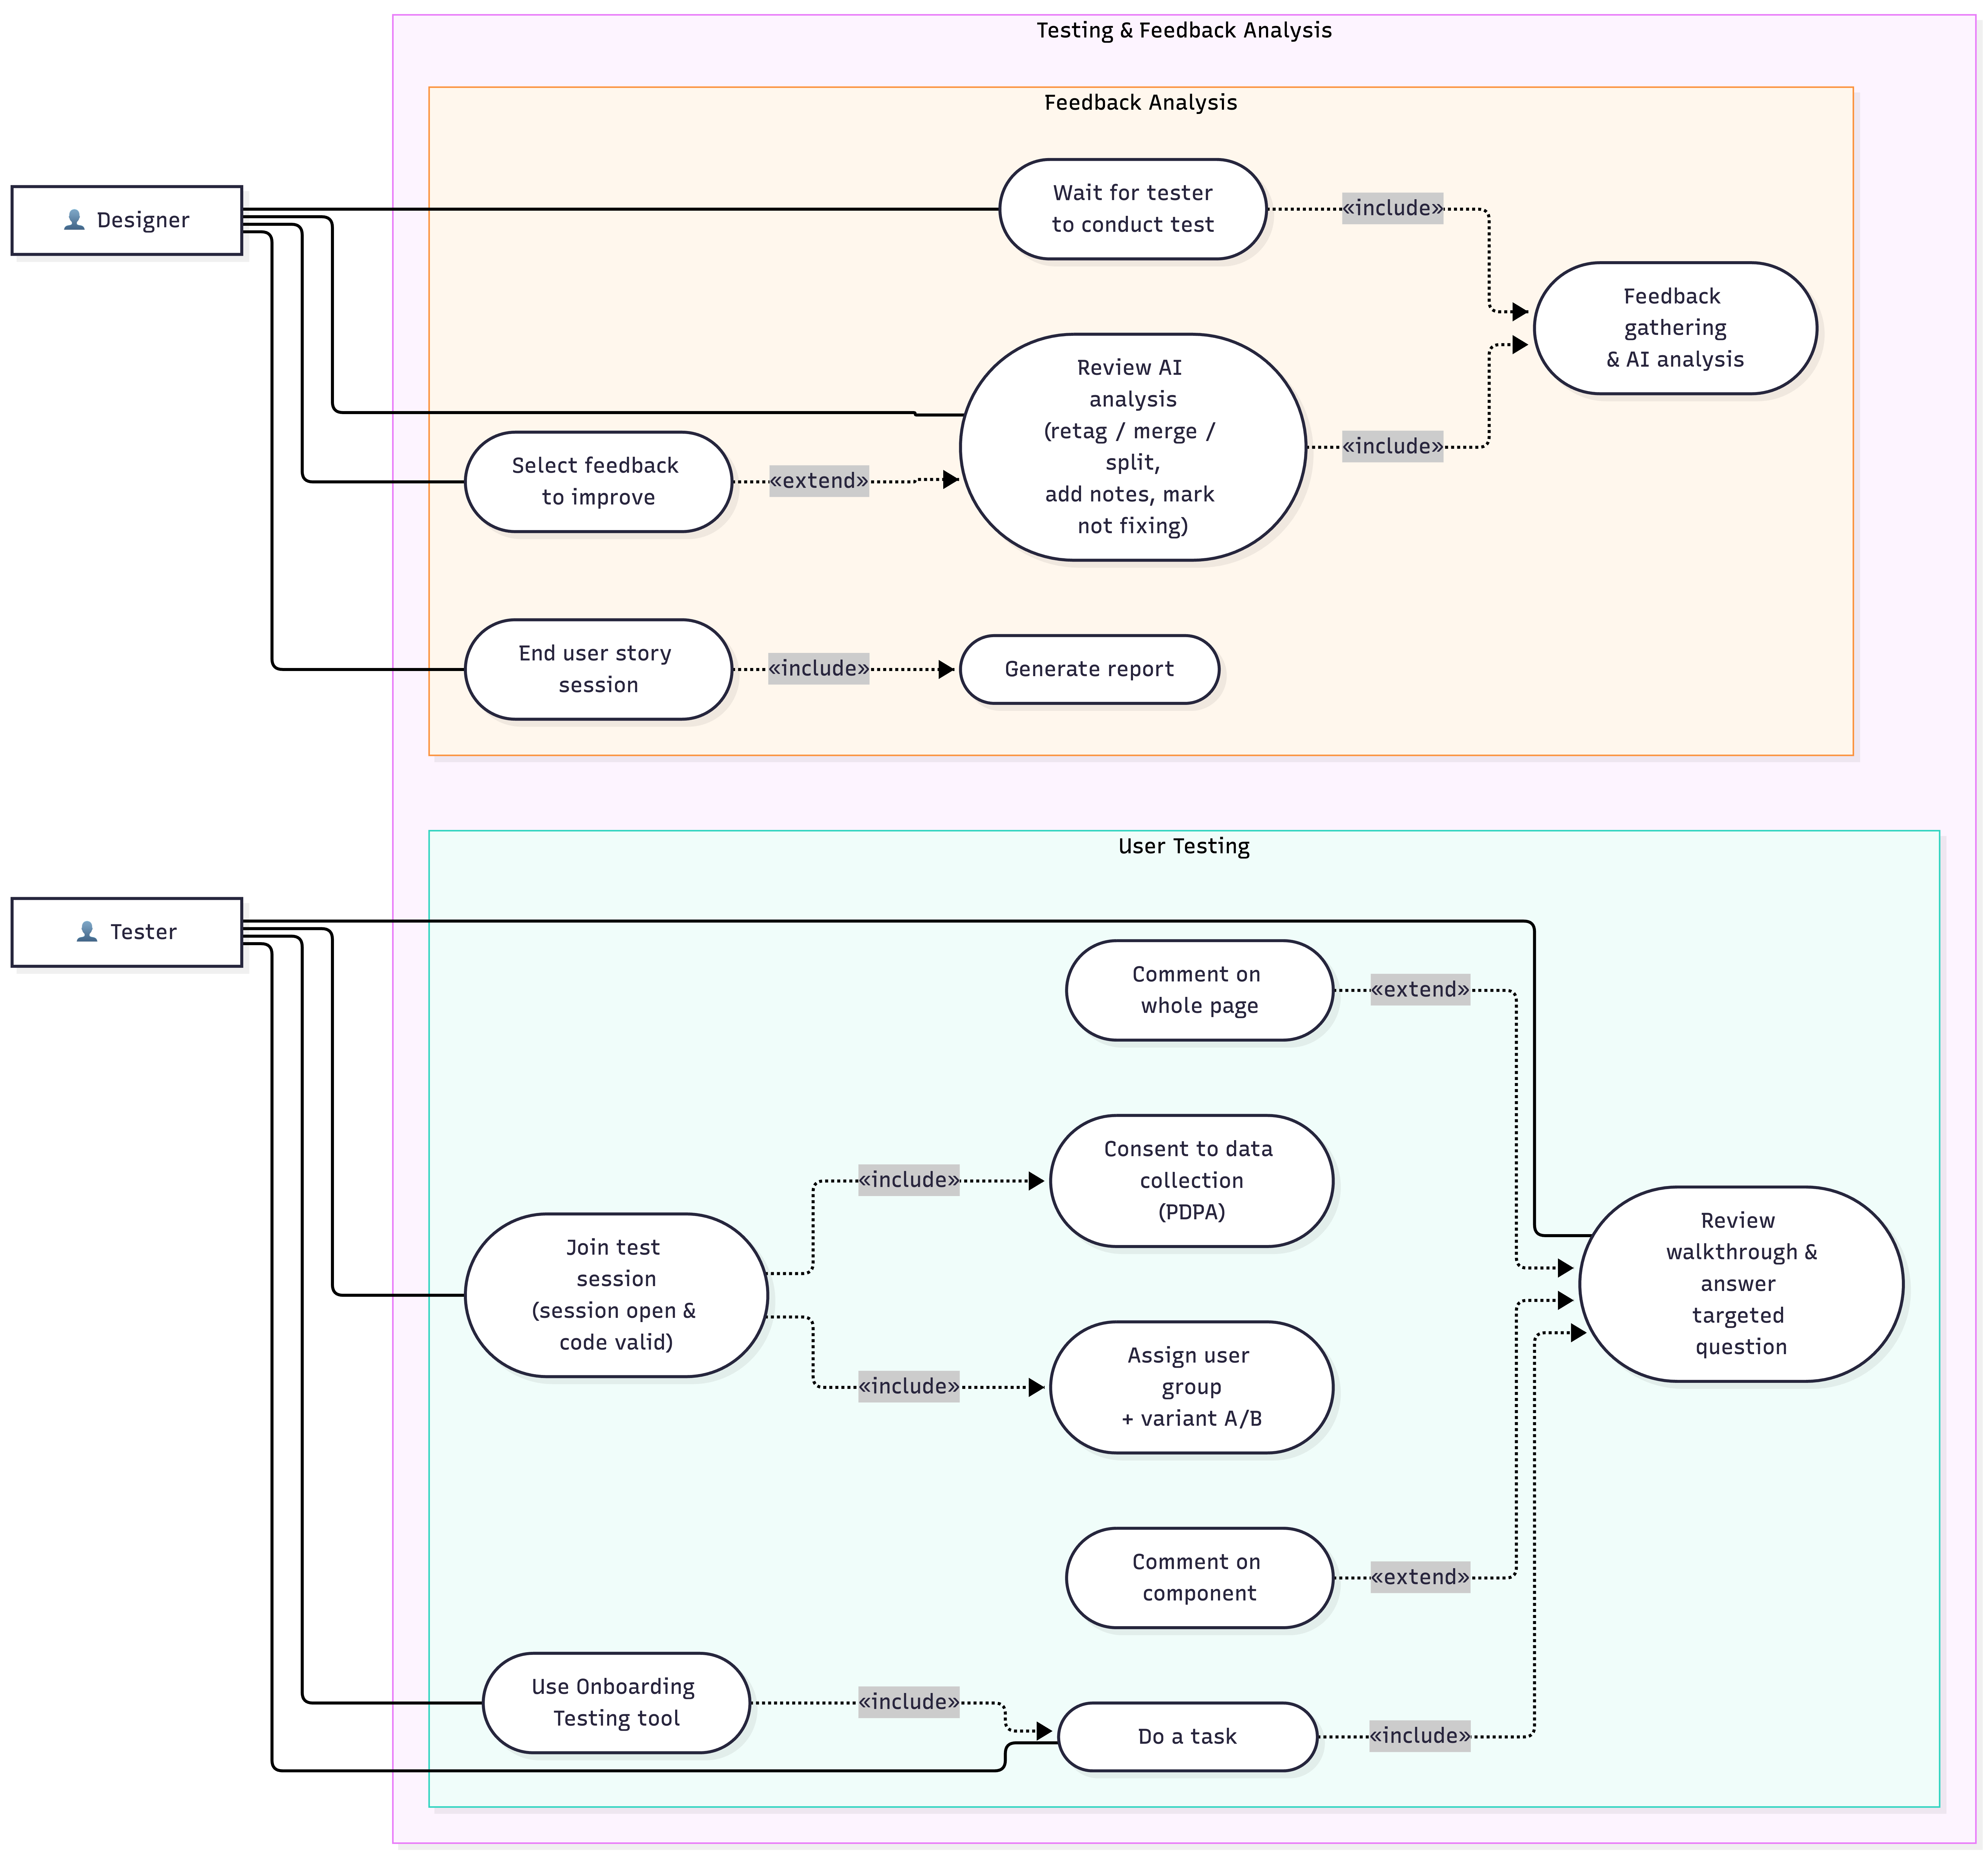
\includegraphics[
      width=0.6\textheight,
      height=\linewidth,
      keepaspectratio,
      origin=c
    ]{figures/ch3-methodology/UC-3.png}
    \caption{Use case diagram for Testing session and Feedback analysis}
    \label{fig:UC-3}
    \thaijustify{ภาพแสดง Use Case ของกระบวนการทดสอบและวิเคราะห์ Feedback โดย Tester เข้าร่วมการทดสอบ ทำภารกิจ และให้ความคิดเห็น ขณะที่ Designer รวบรวมและตรวจสอบผลการทดสอบ วิเคราะห์ Feedback ด้วย AI และเลือกประเด็นเพื่อนำไปปรับปรุงส่วนต่อประสานผู้ใช้}
  \end{figure}
  \subsubsection{Client, Developer, and Project Manager: Project view and Report}
  \begin{figure}[H]
    \centering
    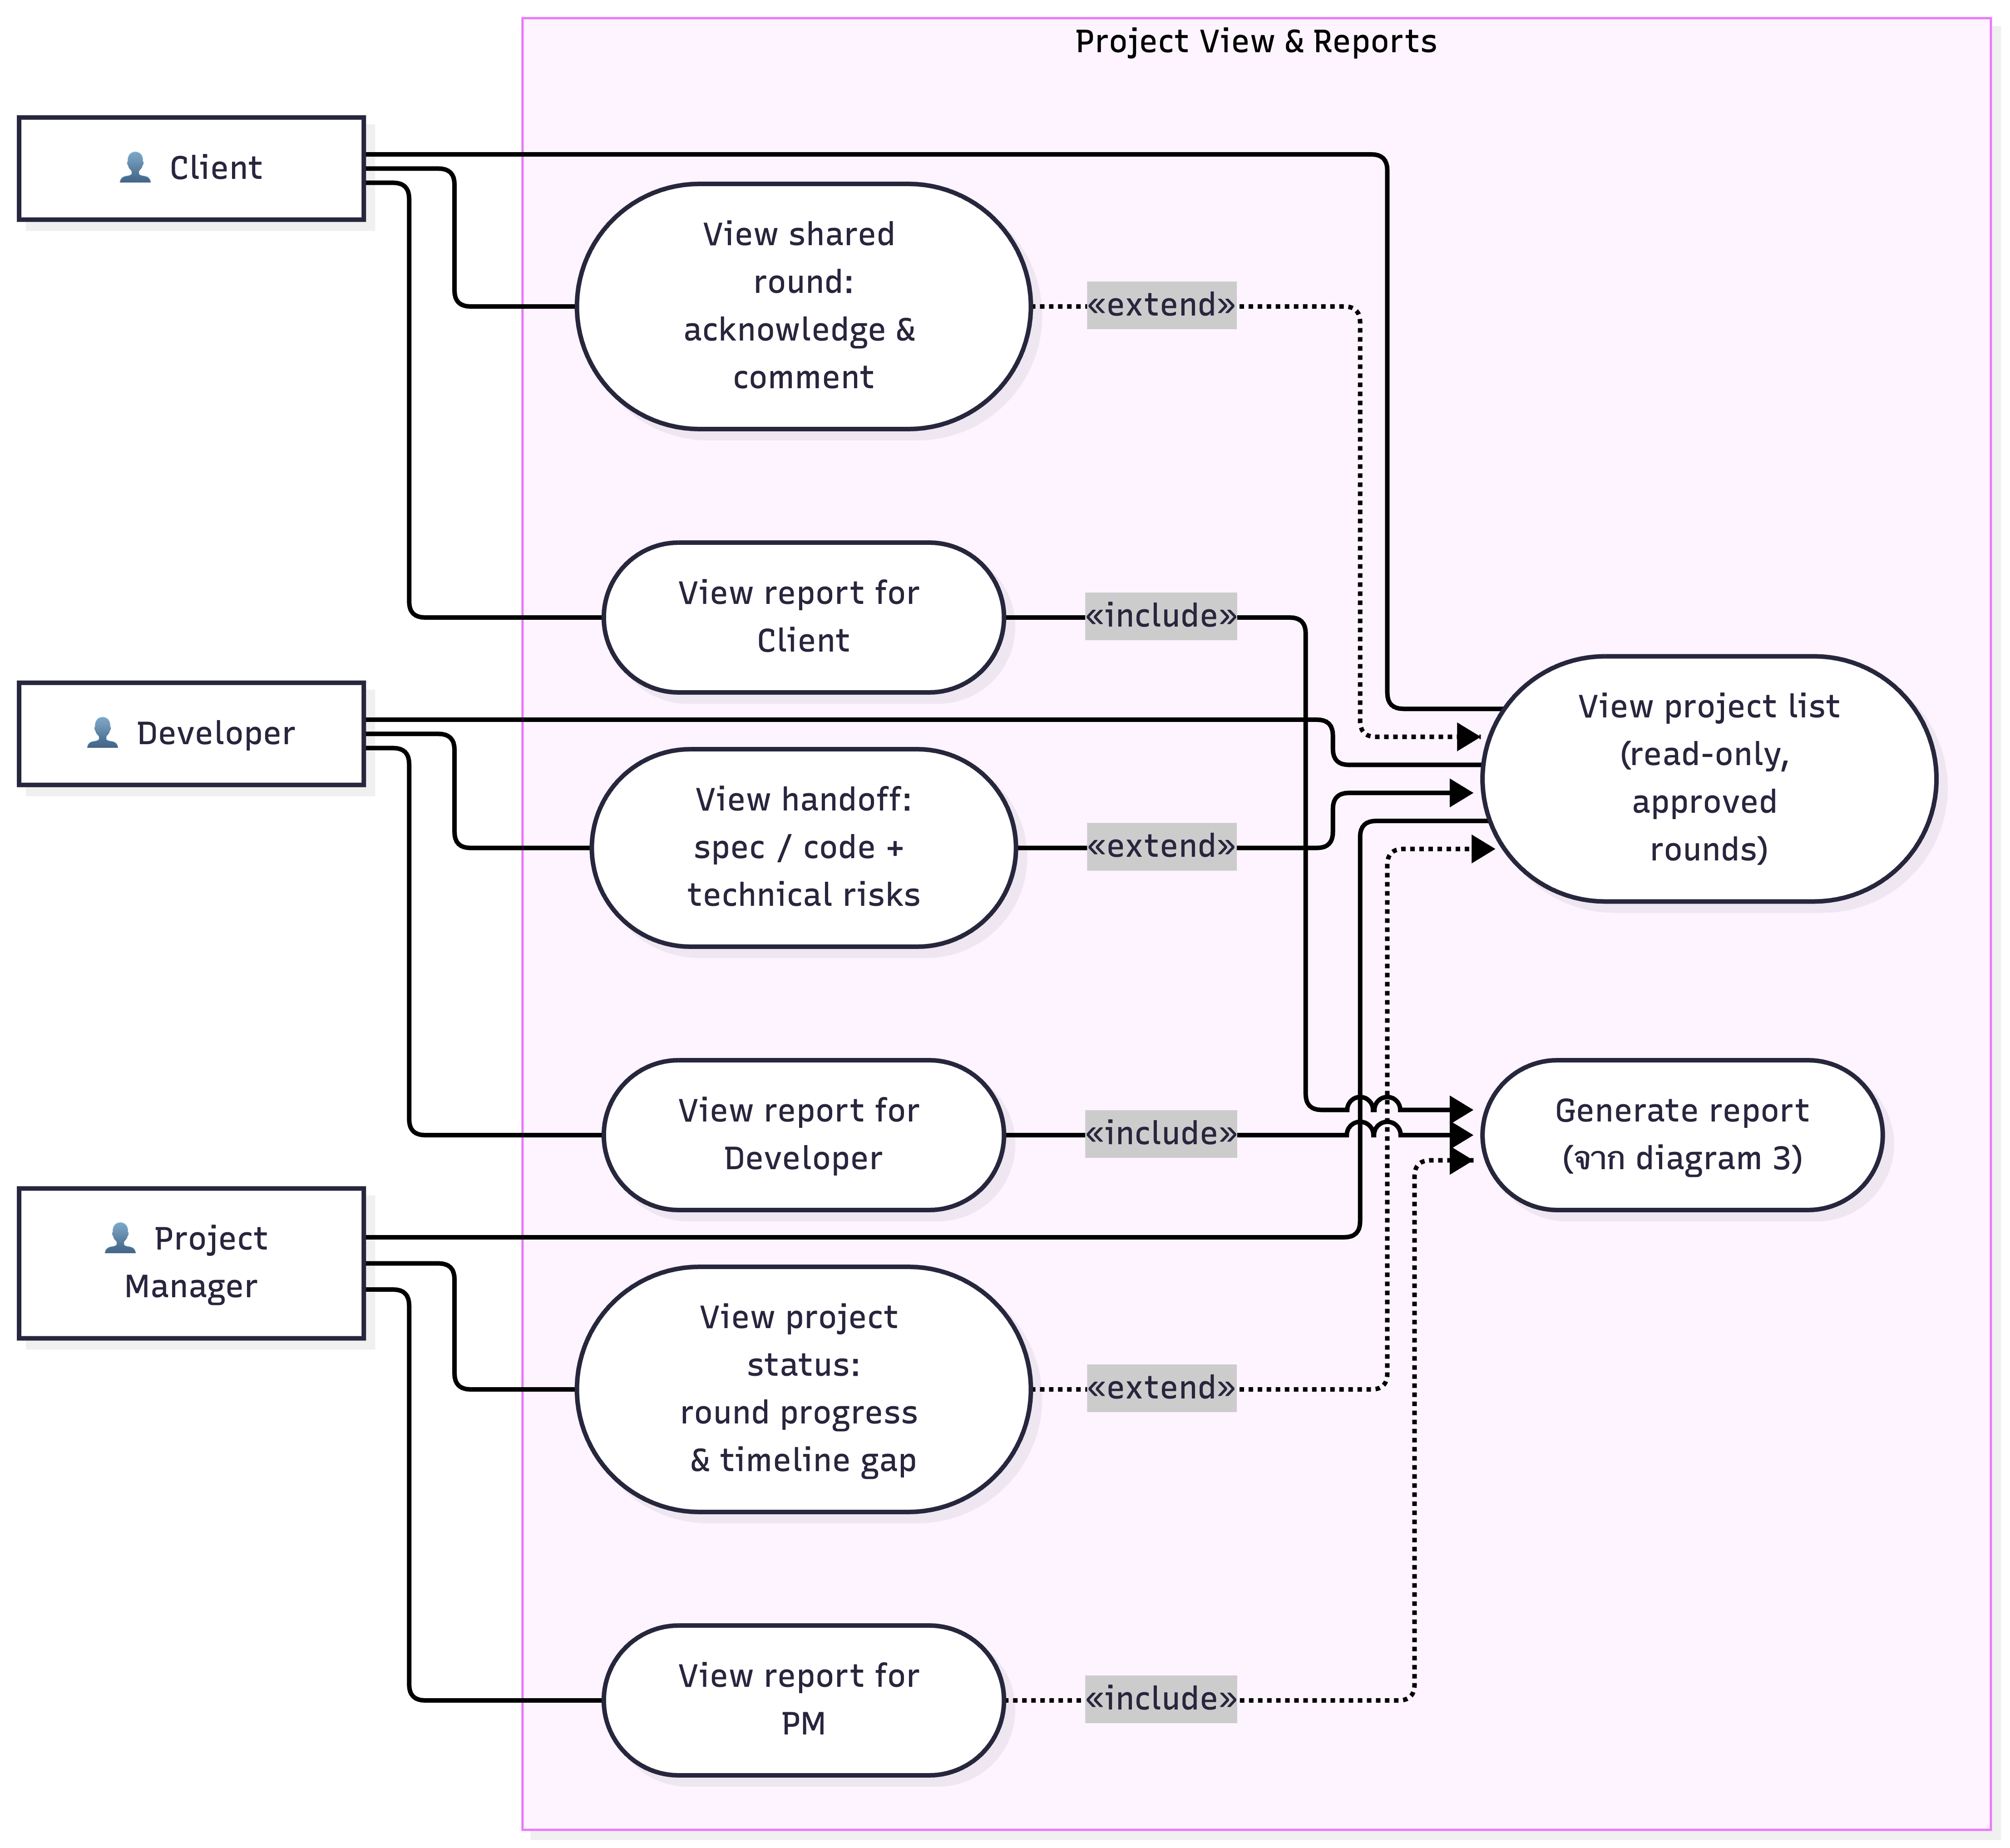
\includegraphics[
      width=0.6\textheight,
      height=\linewidth,
      keepaspectratio,
      origin=c
    ]{figures/ch3-methodology/UC-4.png}
    \caption{Use case diagram for Project view and Report}
    \label{fig:UC-4}
    \thaijustify{
      ภาพแสดง Use Case ของการดูโครงการและรายงาน โดย ผู้ใช้งาน, นักพัฒนา และ ผู้ดูแลโครงการ สามารถดูข้อมูลโครงการที่ได้รับอนุมัติและข้อมูลที่เกี่ยวข้องตามบทบาท รวมถึงดูรายงานที่สร้างจากผลการทดสอบและ Feedback
    }
  \end{figure}
\end{samepage}

\subsection{Sequence Diagram}
\thaijustify{
  \todo{Sequence diagram ของกระบวนการหลัก เช่น การสร้าง two-alternative UI และการทดสอบ}
}

\subsection{ER Diagram}\label{sec:er-diagram}
\thaijustify{
  ฐานข้อมูลของแพลตฟอร์มใช้ PostgreSQL และกำหนดโครงสร้างผ่าน Prisma schema ประกอบด้วย 34 ตารางและ 25 ชนิดข้อมูลแบบ enum เพื่อให้อ่านง่าย จึงแบ่ง ER diagram ออกเป็นสี่กลุ่มตามส่วนของระบบ (รูปที่~\ref{fig:er-workspace-project} ถึง~\ref{fig:er-analysis-report}) ในแต่ละตารางแสดง primary key (PK), foreign key (FK) และคอลัมน์หลักบางส่วน ส่วนตารางสีเทาเป็นตารางจากกลุ่มอื่นที่แสดงไว้เพื่อให้เห็นความสัมพันธ์
}
\thaijustify{
  \textbf{ผู้ใช้ workspace และโปรเจกต์ (รูปที่~\ref{fig:er-workspace-project}):} ผู้ใช้ (User) เข้าสู่ระบบผ่านบัญชีภายนอก (Account) และได้รับ refresh token ที่เก็บเป็นค่า hash แยกตามกลุ่มของการเข้าสู่ระบบ (familyId) ผู้ใช้สร้างหรือได้รับเชิญเข้า workspace โดยมีบทบาท ADMIN หรือ MEMBER (WorkspaceMember) ภายใน workspace มีหลายโปรเจกต์ (Project) และสมาชิกแต่ละคนมีบทบาทในโปรเจกต์ (ProjectMember) ได้แก่ Designer, Project Manager, Client และ Developer แต่ละโปรเจกต์มีความต้องการทางการออกแบบ (DesignIntent) หนึ่งชุด มี persona ได้หลายรายการ (UserPersona) และมีบันทึกกิจกรรม (AuditLog) สำหรับตรวจสอบย้อนหลัง
}
\thaijustify{
  \textbf{การออกแบบและการสร้าง UI ด้วย AI (รูปที่~\ref{fig:er-design-generation}):} โปรเจกต์มี user story (UserStory) ที่นักออกแบบเขียนเองหรือให้ AI ร่าง (StoryGeneration) แต่ละรอบการออกแบบ (DesignRound) อ้างอิง user story หนึ่งเรื่อง และอ้างอิงรอบก่อนหน้าได้ (parentRoundId) เมื่อสั่งสร้าง UI ระบบสร้างงาน (GenerationJob) ที่เก็บ prompt และจำนวน variant ไว้ ผลลัพธ์คือ UI variant (UIVariant) ซึ่งเก็บ HTML และผลการตรวจการเข้าถึง เมื่อนักออกแบบปรับแก้ variant ระบบสร้าง variant ใหม่ที่อ้างอิงฉบับเดิม (parentVariantId) จึงย้อนดูประวัติแต่ละเวอร์ชันได้
}
\thaijustify{
  \textbf{เซสชันการทดสอบ (รูปที่~\ref{fig:er-testing}):} เซสชันการทดสอบ (TestSession) ผูกกับรอบการออกแบบหนึ่งรอบ และเลือก variant ที่ใช้ทดสอบผ่านตาราง SessionVariant ผู้เข้าร่วมทดสอบ (SessionParticipant) ได้รับลิงก์เชิญที่เก็บเป็นค่า hash และต้องให้ความยินยอมตาม PDPA ก่อนเริ่ม ซึ่งบันทึกไว้ใน ConsentRecord พร้อมเวอร์ชันของข้อความที่ยินยอม ระหว่างทำภารกิจ (TestTask) ระบบบันทึกการทำภารกิจแต่ละครั้ง (TaskRun) พฤติกรรมการใช้งาน (InteractionEvent) และข้อเสนอแนะ (Feedback) ซึ่งระบุได้ว่าเป็นความเห็นต่อ component หรือต่อทั้งหน้าจอ
}
\thaijustify{
  \textbf{การวิเคราะห์ข้อเสนอแนะและรายงาน (รูปที่~\ref{fig:er-analysis-report}):} ผลการวิเคราะห์ข้อเสนอแนะด้วย AI เก็บใน FeedbackAnalysis และแยกเป็นประเด็น (FeedbackTheme) ที่เชื่อมกับข้อเสนอแนะต้นทางผ่าน ThemeFeedback นักออกแบบรวม แยก หรือตัดสินใจไม่แก้ไขประเด็นได้ ทุกการตัดสินใจถูกบันทึกใน DesignDecision และประเด็นที่เลือกไปปรับปรุงเชื่อมกับรอบการออกแบบถัดไปผ่าน RoundFeedbackLink ทำให้สืบย้อนได้ว่าการเปลี่ยนแปลงแต่ละครั้งมาจากข้อเสนอแนะใด ผู้มีส่วนได้ส่วนเสียแสดงความเห็นและรับทราบรอบที่อนุมัติแล้วได้ (RoundComment, RoundAcknowledgement) และระบบสร้างรายงาน (Report) แยกตามบทบาท
}

\begin{figure}[p]
  \centering
  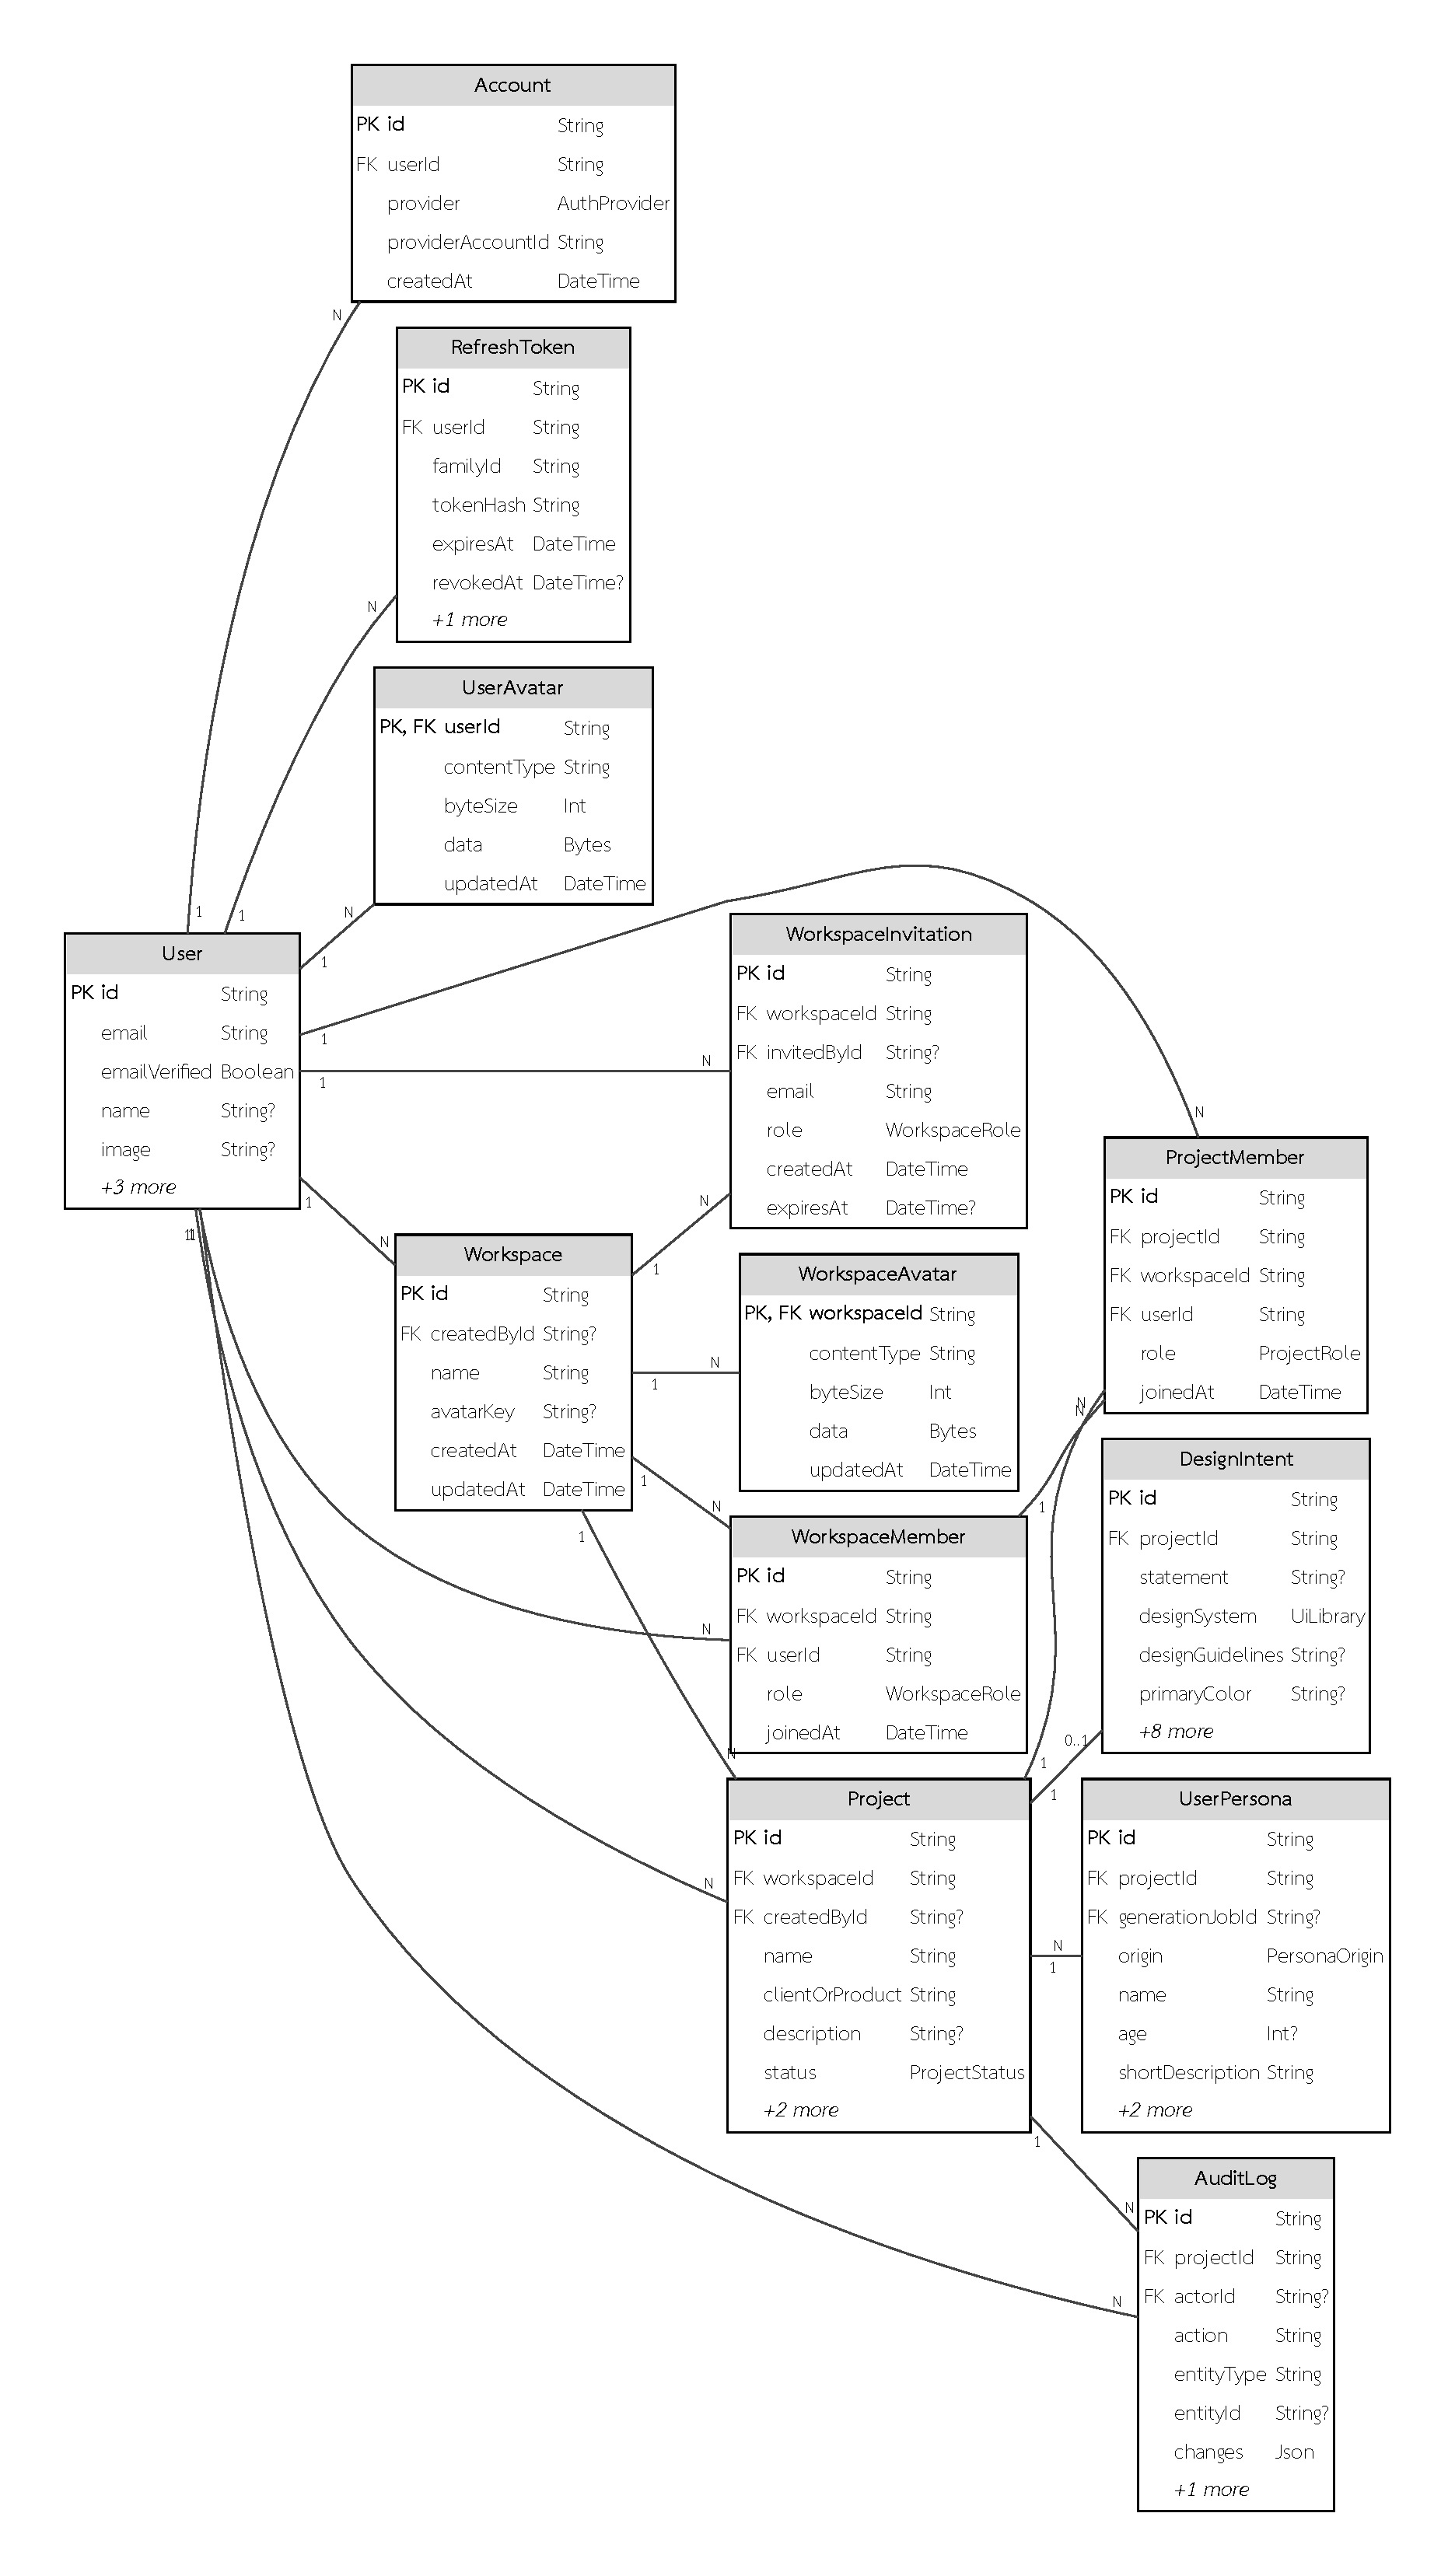
\includegraphics[width=\linewidth,height=0.88\textheight,keepaspectratio]{figures/ch3-methodology/er-workspace-project.pdf}
  \caption{ER diagram ส่วนผู้ใช้ workspace และโปรเจกต์}
  \label{fig:er-workspace-project}
\end{figure}
\begin{figure}[p]
  \centering
  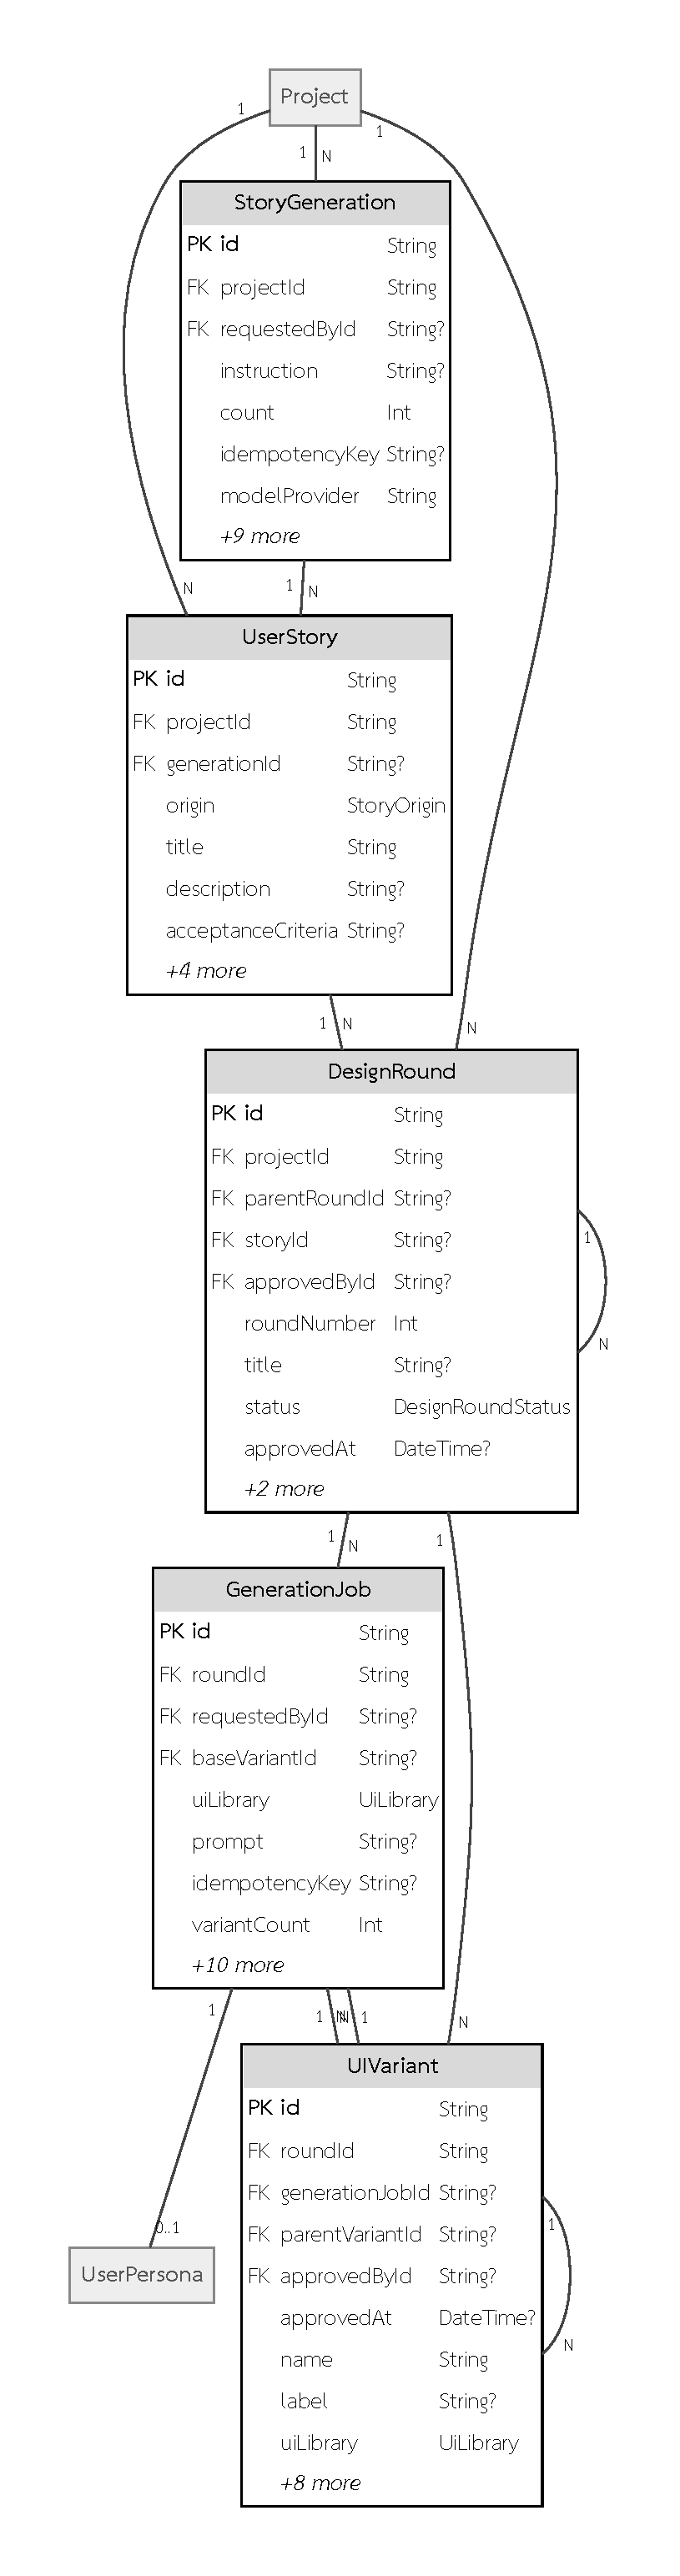
\includegraphics[width=\linewidth,height=0.88\textheight,keepaspectratio]{figures/ch3-methodology/er-design-generation.pdf}
  \caption{ER diagram ส่วนการออกแบบและการสร้าง UI ด้วย AI}
  \label{fig:er-design-generation}
\end{figure}
\begin{figure}[p]
  \centering
  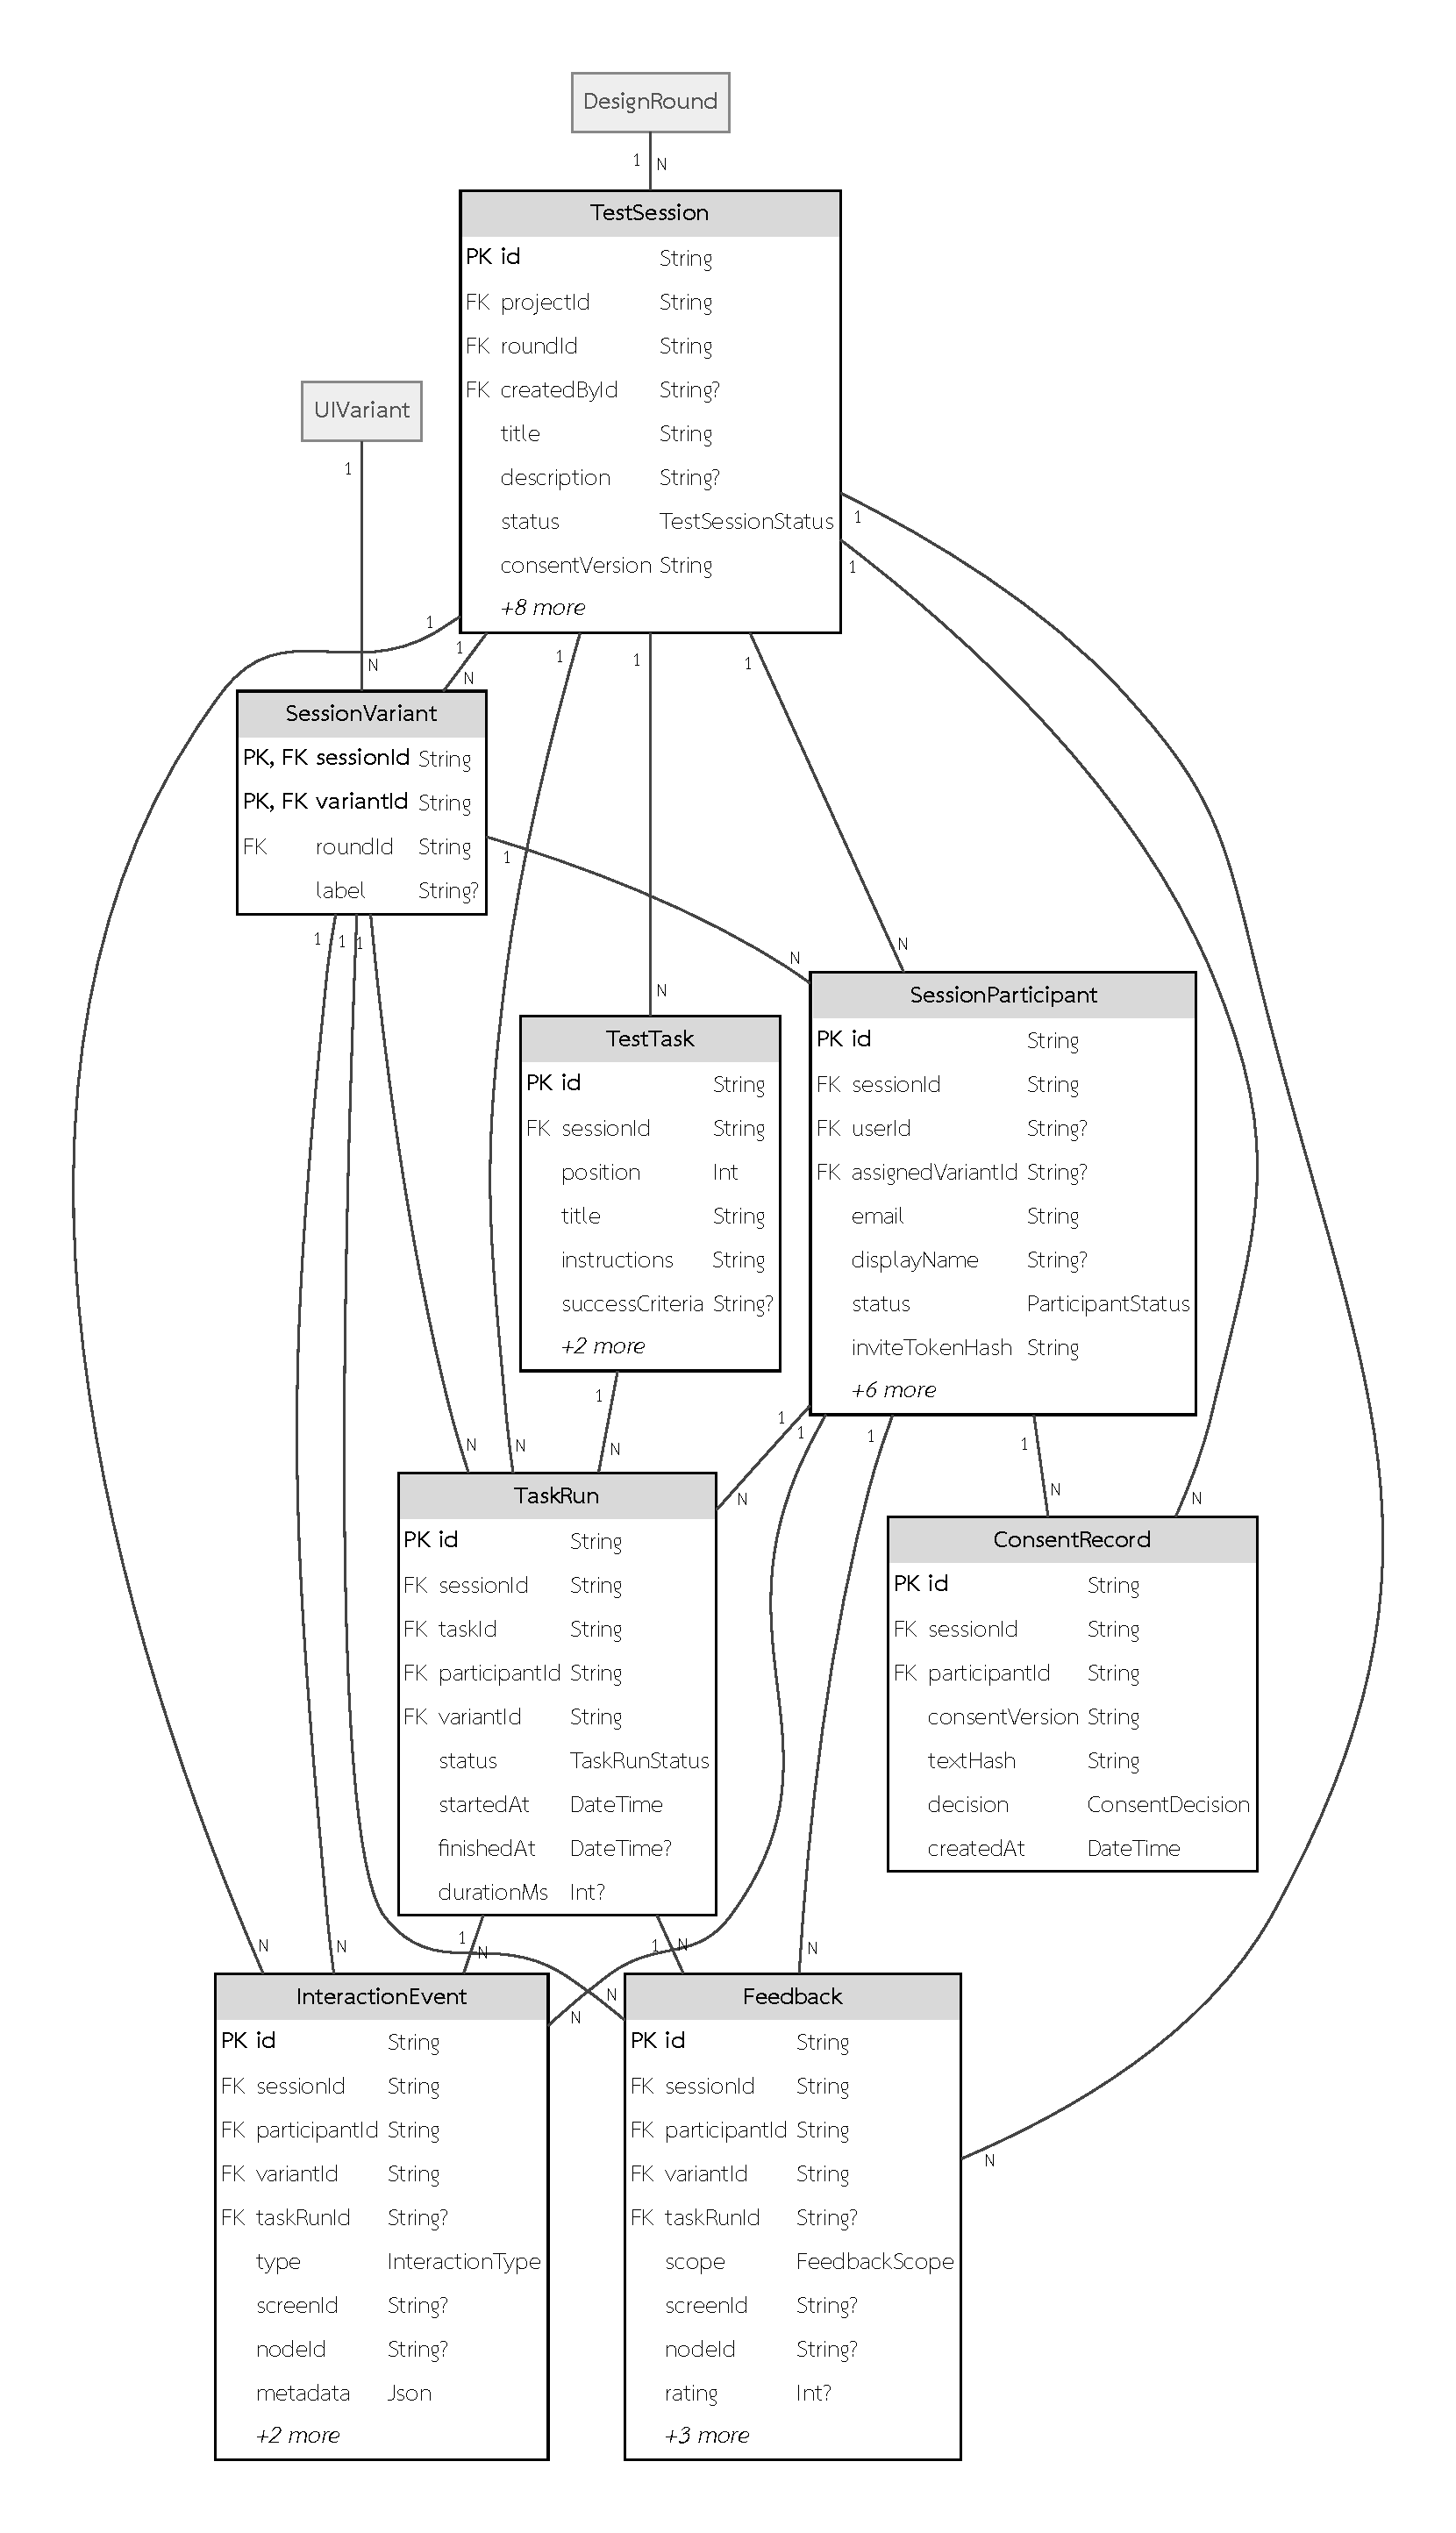
\includegraphics[width=\linewidth,height=0.88\textheight,keepaspectratio]{figures/ch3-methodology/er-testing.pdf}
  \caption{ER diagram ส่วนเซสชันการทดสอบ}
  \label{fig:er-testing}
\end{figure}
\begin{figure}[p]
  \centering
  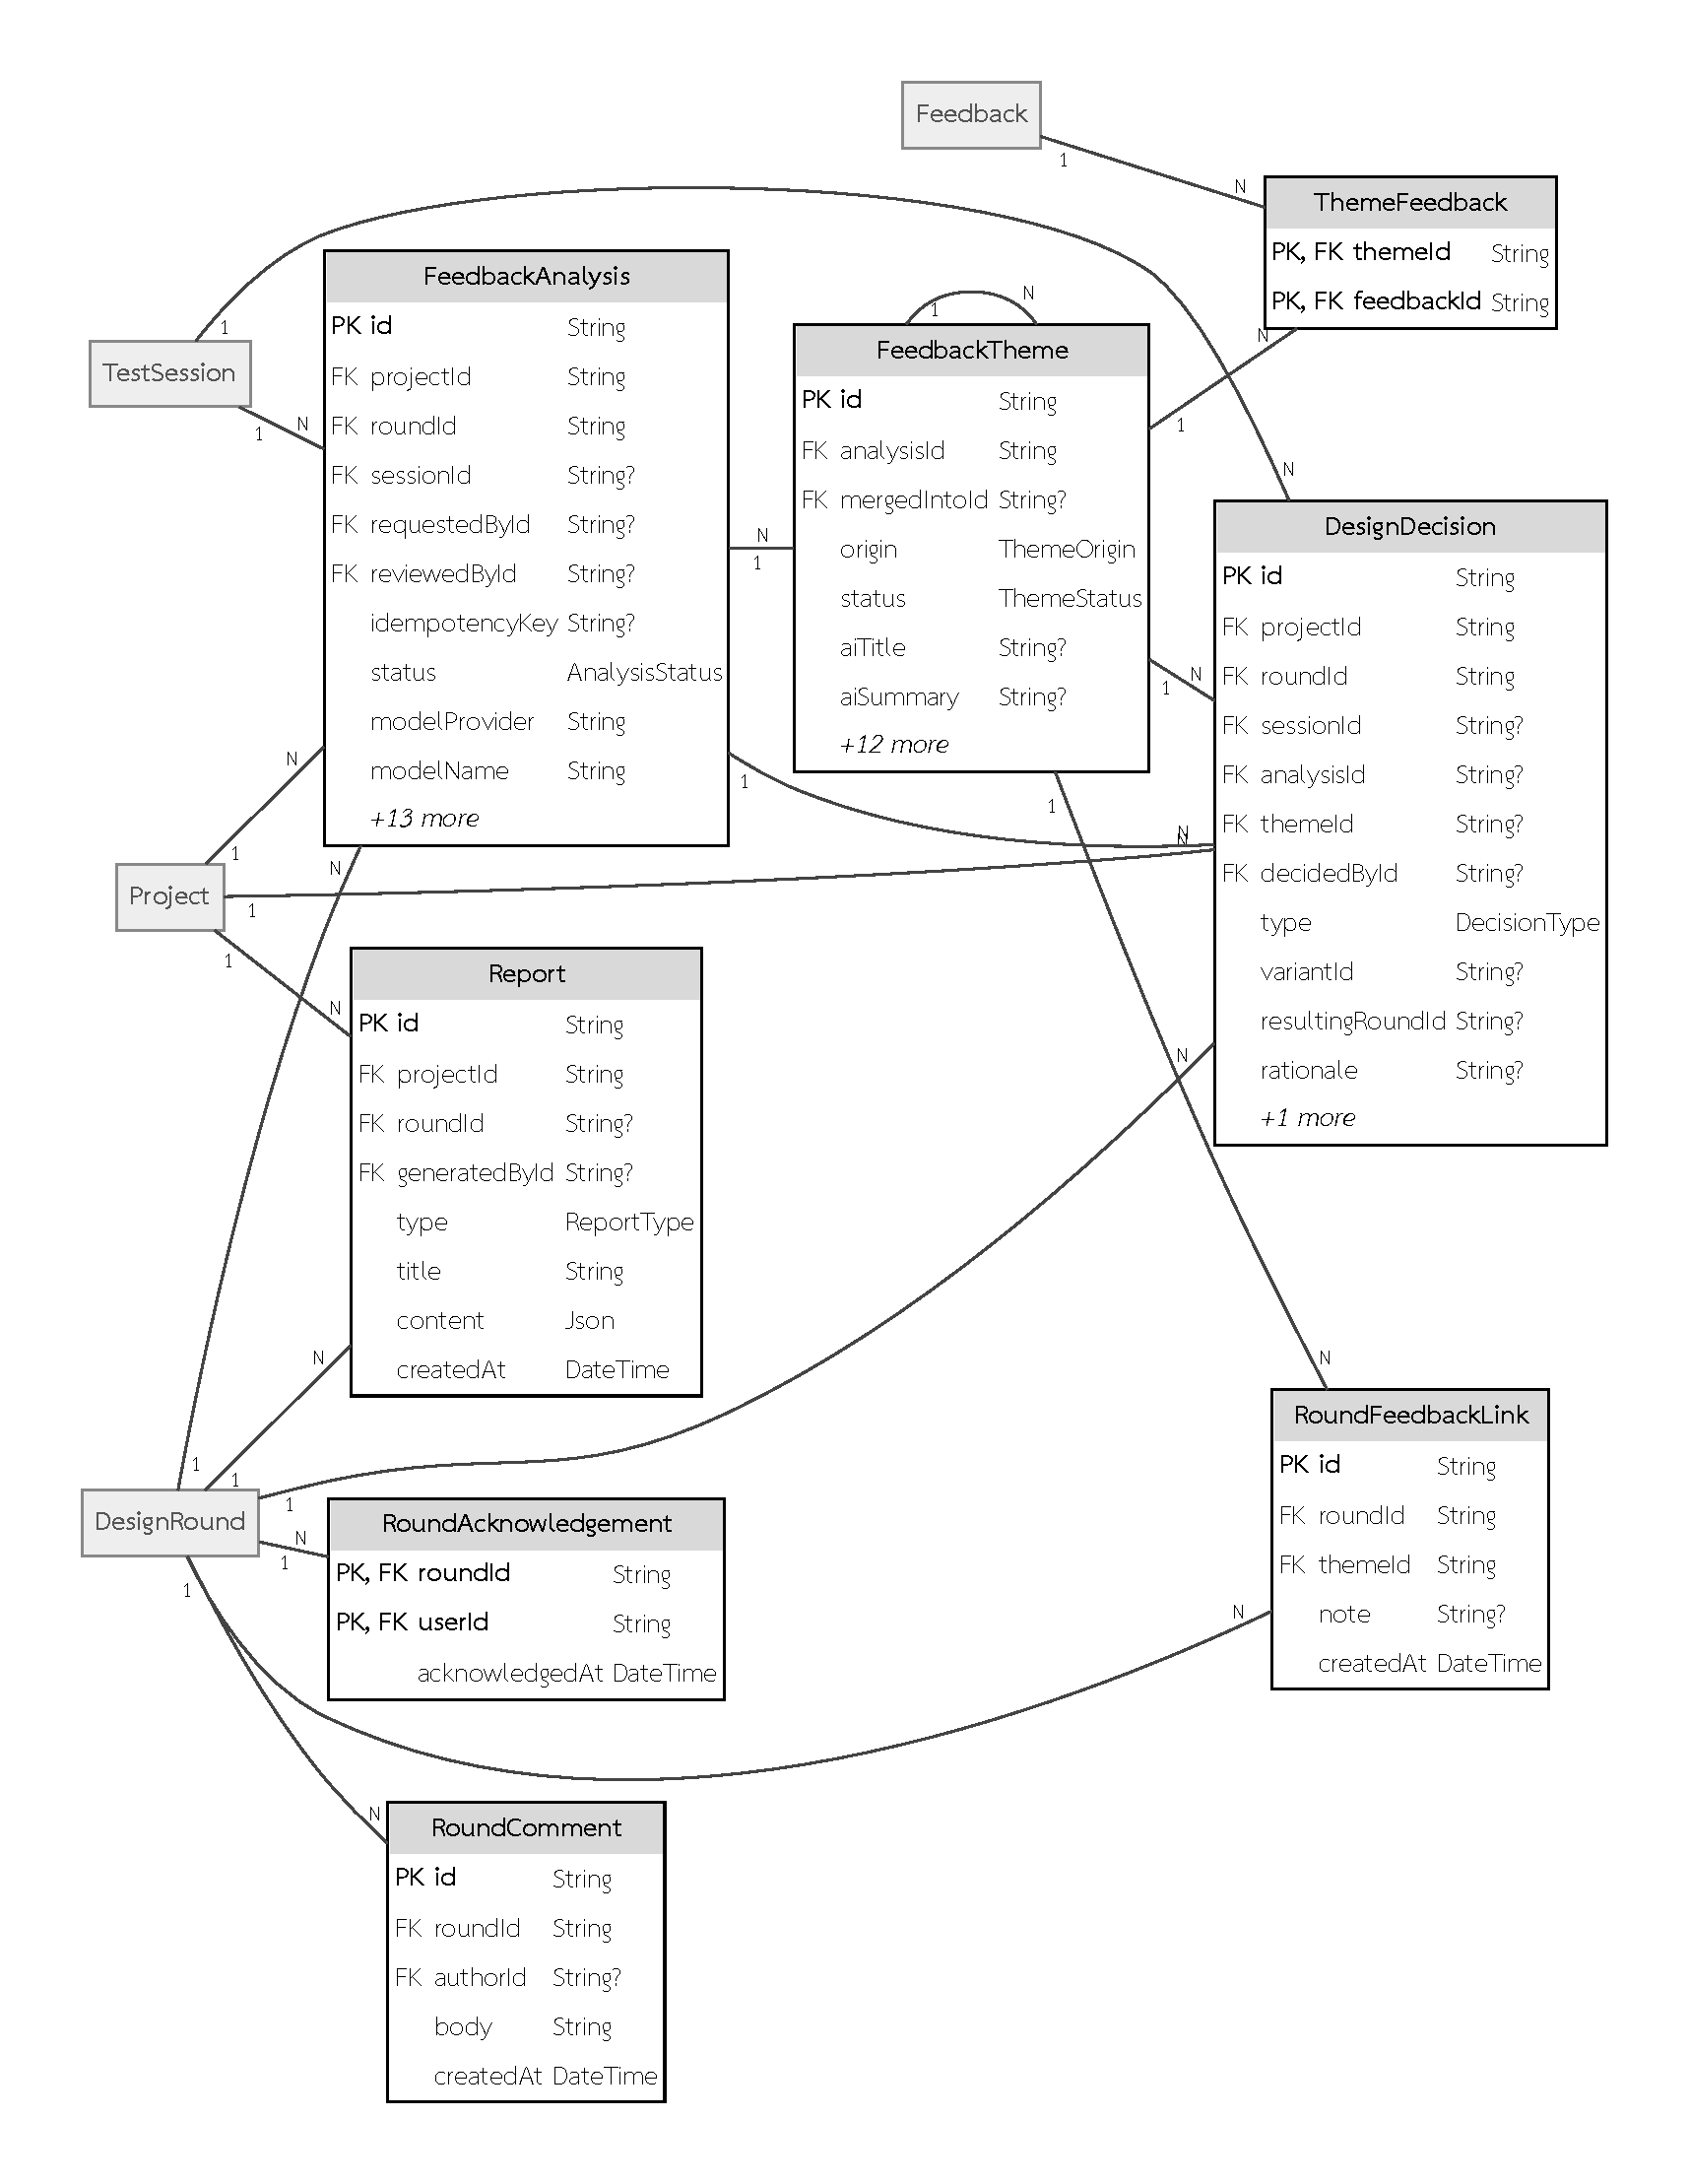
\includegraphics[width=\linewidth,height=0.88\textheight,keepaspectratio]{figures/ch3-methodology/er-analysis-report.pdf}
  \caption{ER diagram ส่วนการวิเคราะห์ข้อเสนอแนะและรายงาน}
  \label{fig:er-analysis-report}
\end{figure}

\subsection{User Flow และแผนผังเว็บไซต์ (Site Map)}
\thaijustify{
  \todo{User flow และ sitemap ให้ตรงกับ hi-fi v2}
}
